\section{Results}
\label{sec:res}

% - 19 classes within 3 groups
The resulting classification of Great Britain identified 19 types of
morphosignatures that can be organised into three macro groups: countryside, suburban low
density development and dense city centres. It is a result of two hierarchical steps
based on K-Means clustering, where the first resulted in seven classes, of which the two
most urban have been further clustered into six and eight lower-level classes (after a removal
of outlier classes). An illustration of the classification in London is shown on Figure
\ref{fig:london} and in Birmingham on Figure \ref{fig:bham}.

\begin{figure}
    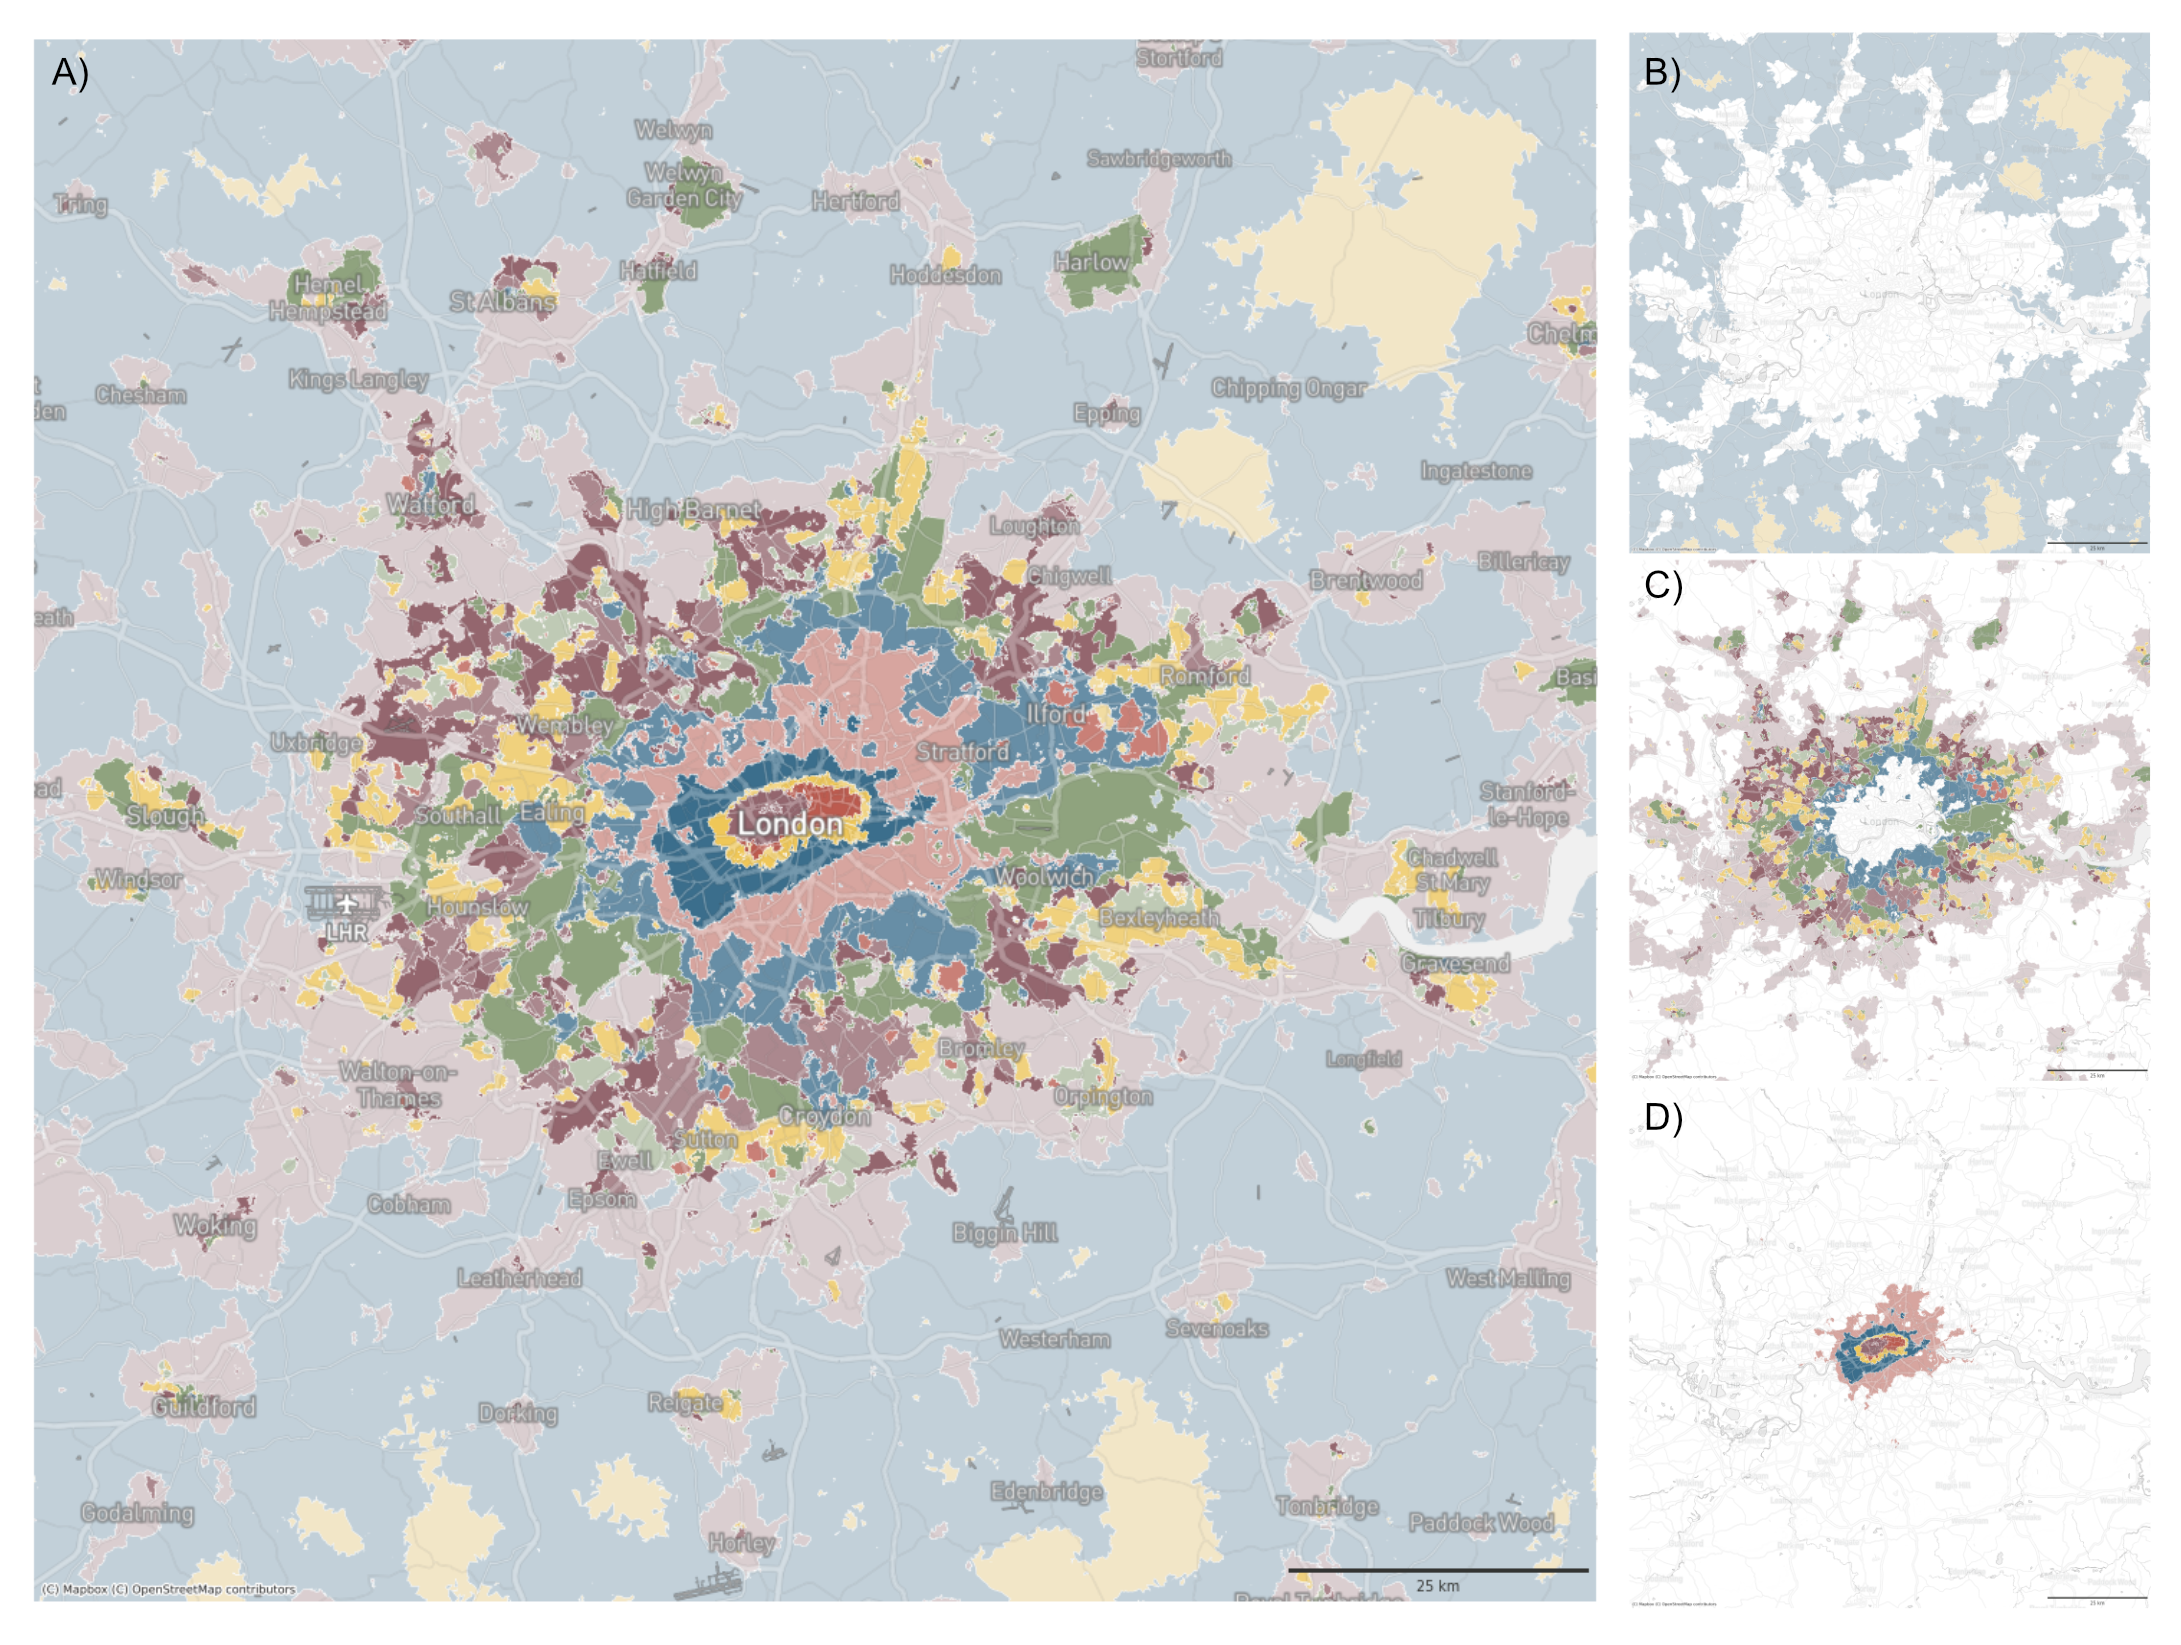
\includegraphics[width=0.75\linewidth, center]{fig/london.png}
    \caption{Morphosignatures in London (A), and their classification into
    top-level macro groups (countryside (B), suburban development (C) and city centres
    (D)).
    Contains OS data © Crown copyright and database right 2021. 
    }
    \label{fig:london}
\end{figure}

% -- countryside --- brief portrait
The countryside macro group is composed of four morphosignature types covering large-scale open
spaces from agricultural land in southern England to vast natural areas of the Scottish
Highlands. The urban development in this group is limited to small villages or hamlets.
All four classes are a result of the first clustering step.

\begin{figure}
    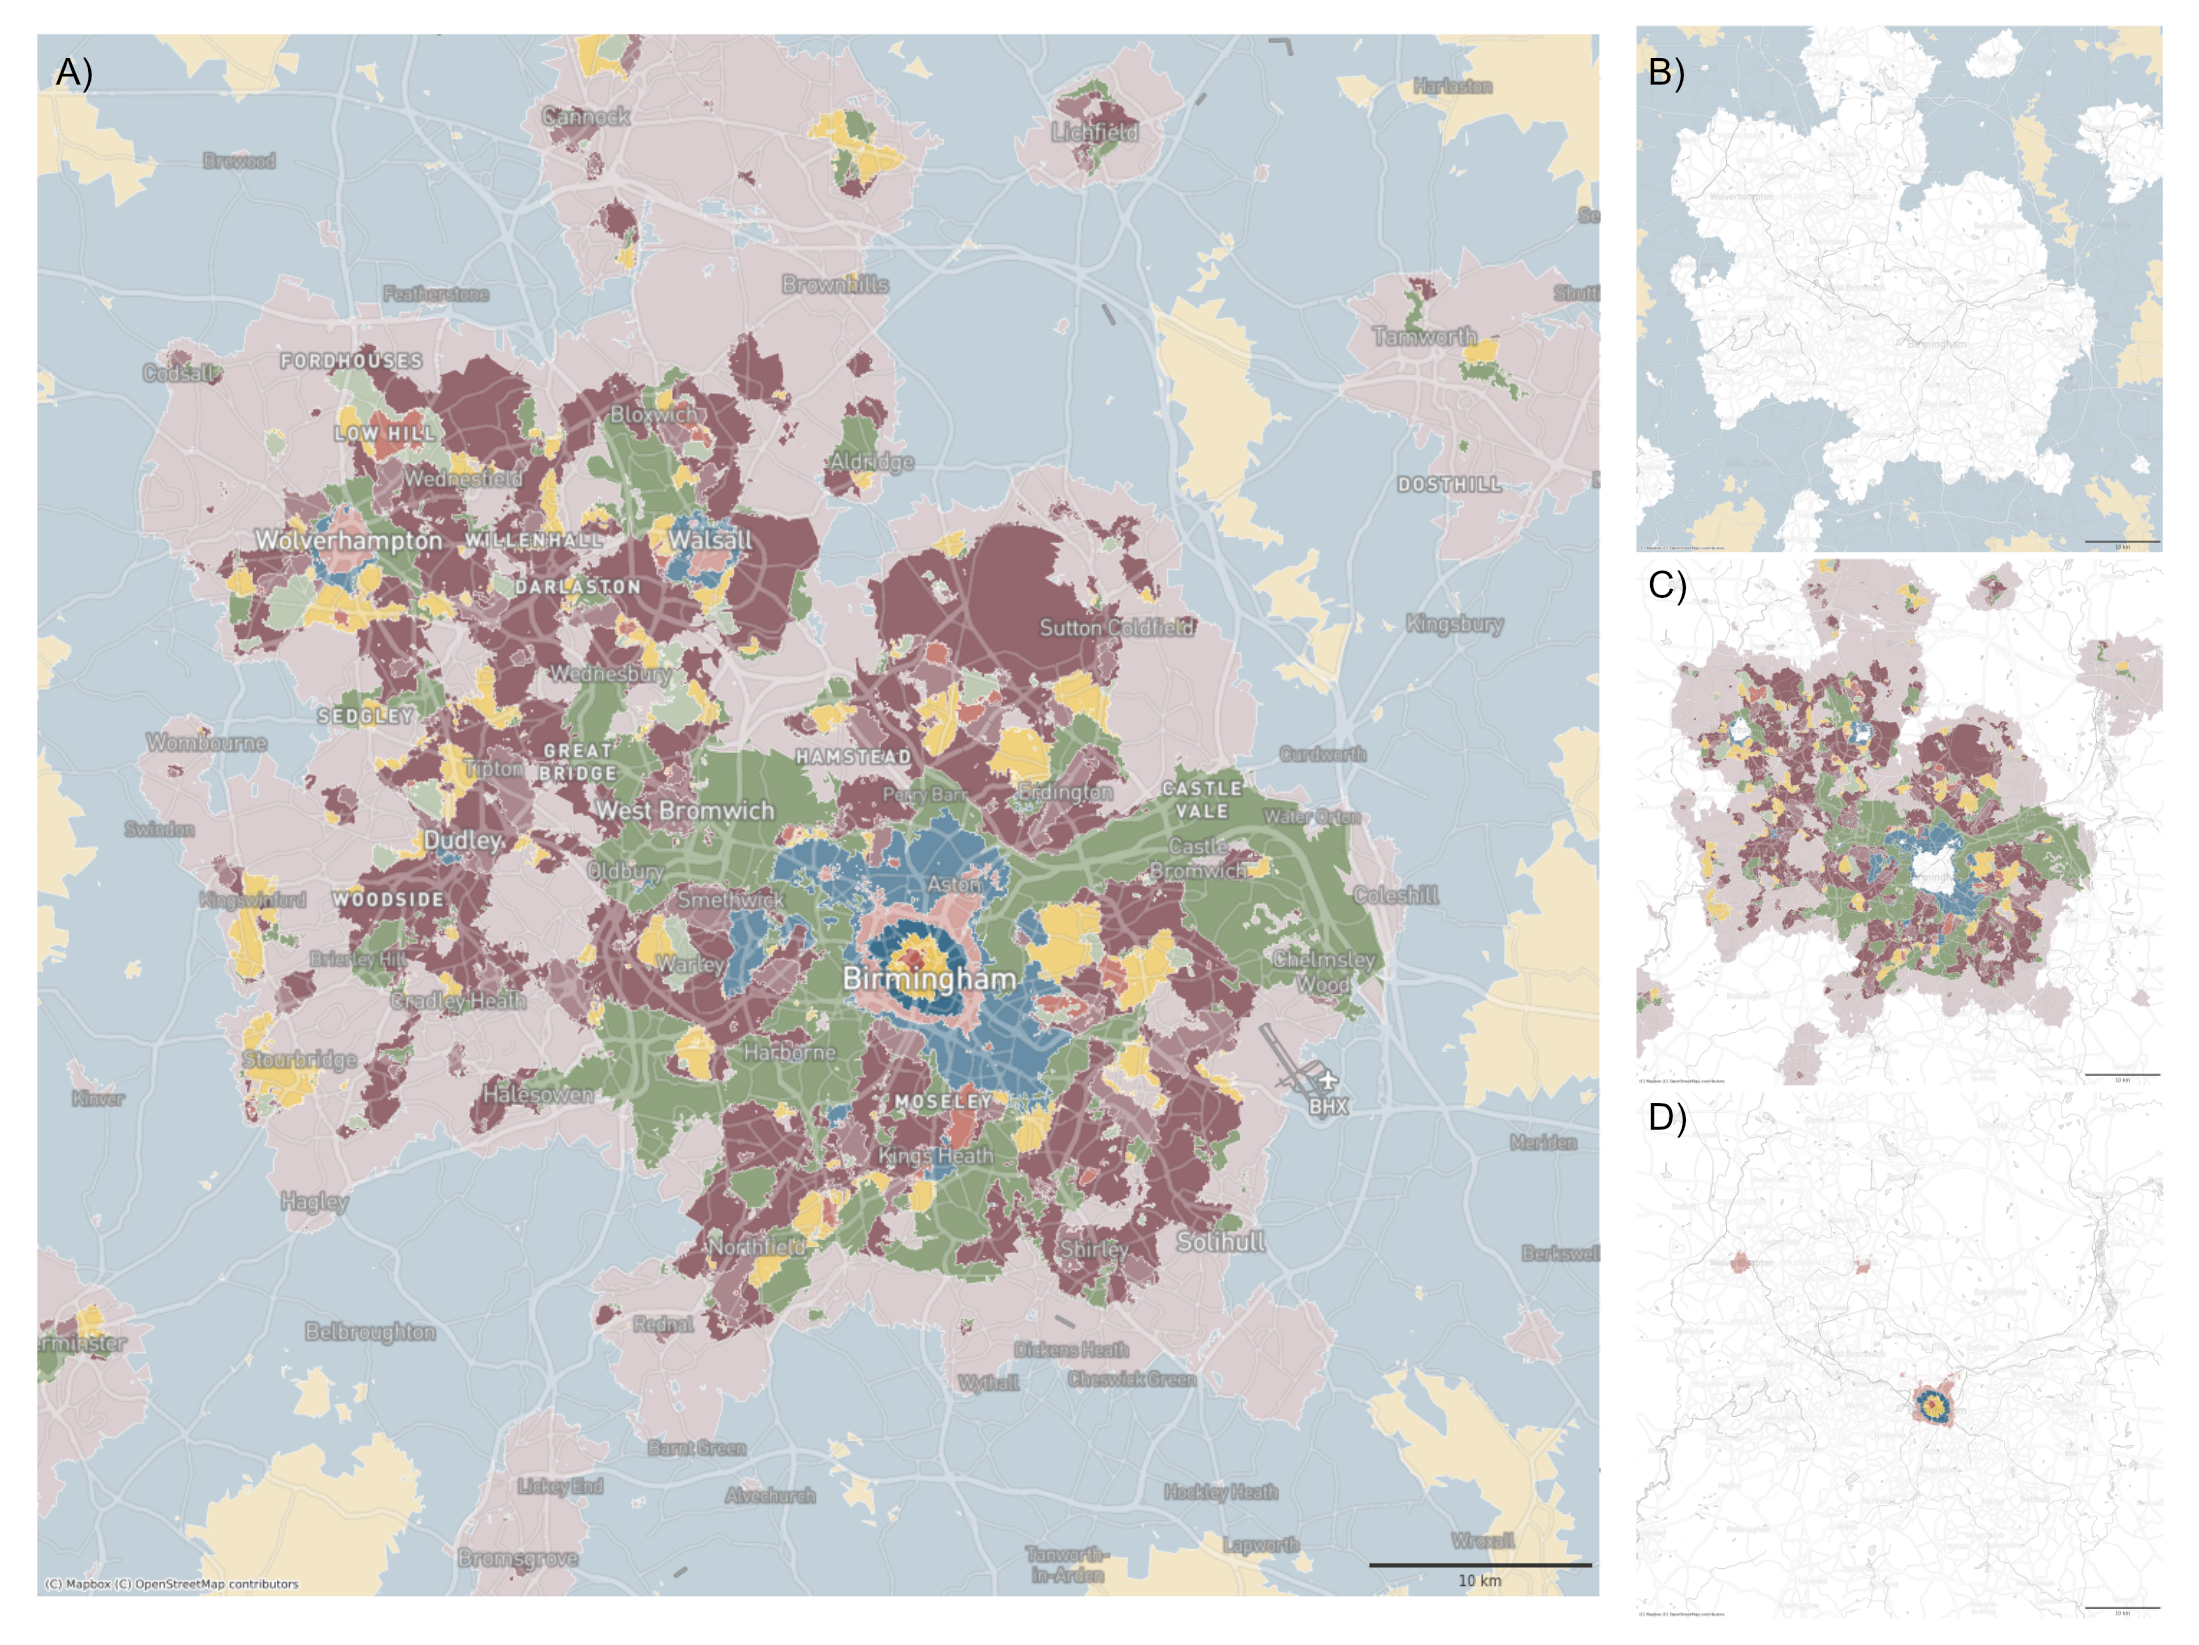
\includegraphics[width=0.75\linewidth, center]{fig/bham.png}
    \caption{Morphosignatures in Birmingham (A), and their classification
    into top-level macro groups (countryside (B), suburban development (C) and city
    centres (D)). Contains OS data © Crown copyright and database right 2021. }
    \label{fig:bham}
\end{figure}

% -- suburbs --- brief portrait
The second macro group covers suburban low-density development areas, taking up most of the
area of british cities. We identify nine types of morphosignatures, originating in two
classes from the first step. The range of types stretches from sparse single-family
housing on the peripheries of cities, planned residential developments of 20th century
to predominantly industrial areas. The types differ in many aspects, from the overall
built-up density and related geometry of both enclosed tessellation and enclosures (both
affecting the description via many morphometric characters) to connectivity of street
networks or their solar orientation.


% -- city centres --- brief portrait
Final macro group comprises of dense town and city centres, all originating from the
single top level cluster. These morphosignatures reflect the main hubs of activities in each
larger settlement. In some cases, they are all located in the same central areas, while
in others some local district nodes show up (e.g. Liverpool). All six types can be
arranged according to their level of \textit{urbanity} and tend to form concentric
rings.


% - Concentric character of British centers and centre hierarchy -- from London to
%   Oxford
Two types are exclusive to London's city centre (roughly around Soho as show on Figure
\ref{fig:centres}A) and are not present anywhere else in the whole country. The
remaining are present in other places and their presence can encode the
\textit{urbanity} of each city or town. For example, Birmingham as the second largest
city in the country contains four types of central morphosignatures (Figure
\ref{fig:centres}B), compared to six in London. Scottish capital Edinburgh contains only
three (like many other cities across the country (e.g. Manchester or Glasgow)
illustrated on Figure \ref{fig:centres}C. Smaller cities like Southampton have only two
types (Figure \ref{fig:centres}D) and towns as Oxford are limited to a single central
type (Figure \ref{fig:centres}E). The presence of types is not accidental -- smaller
cities lack the most urban types, while all of them contain the least urban type.

\begin{figure}
    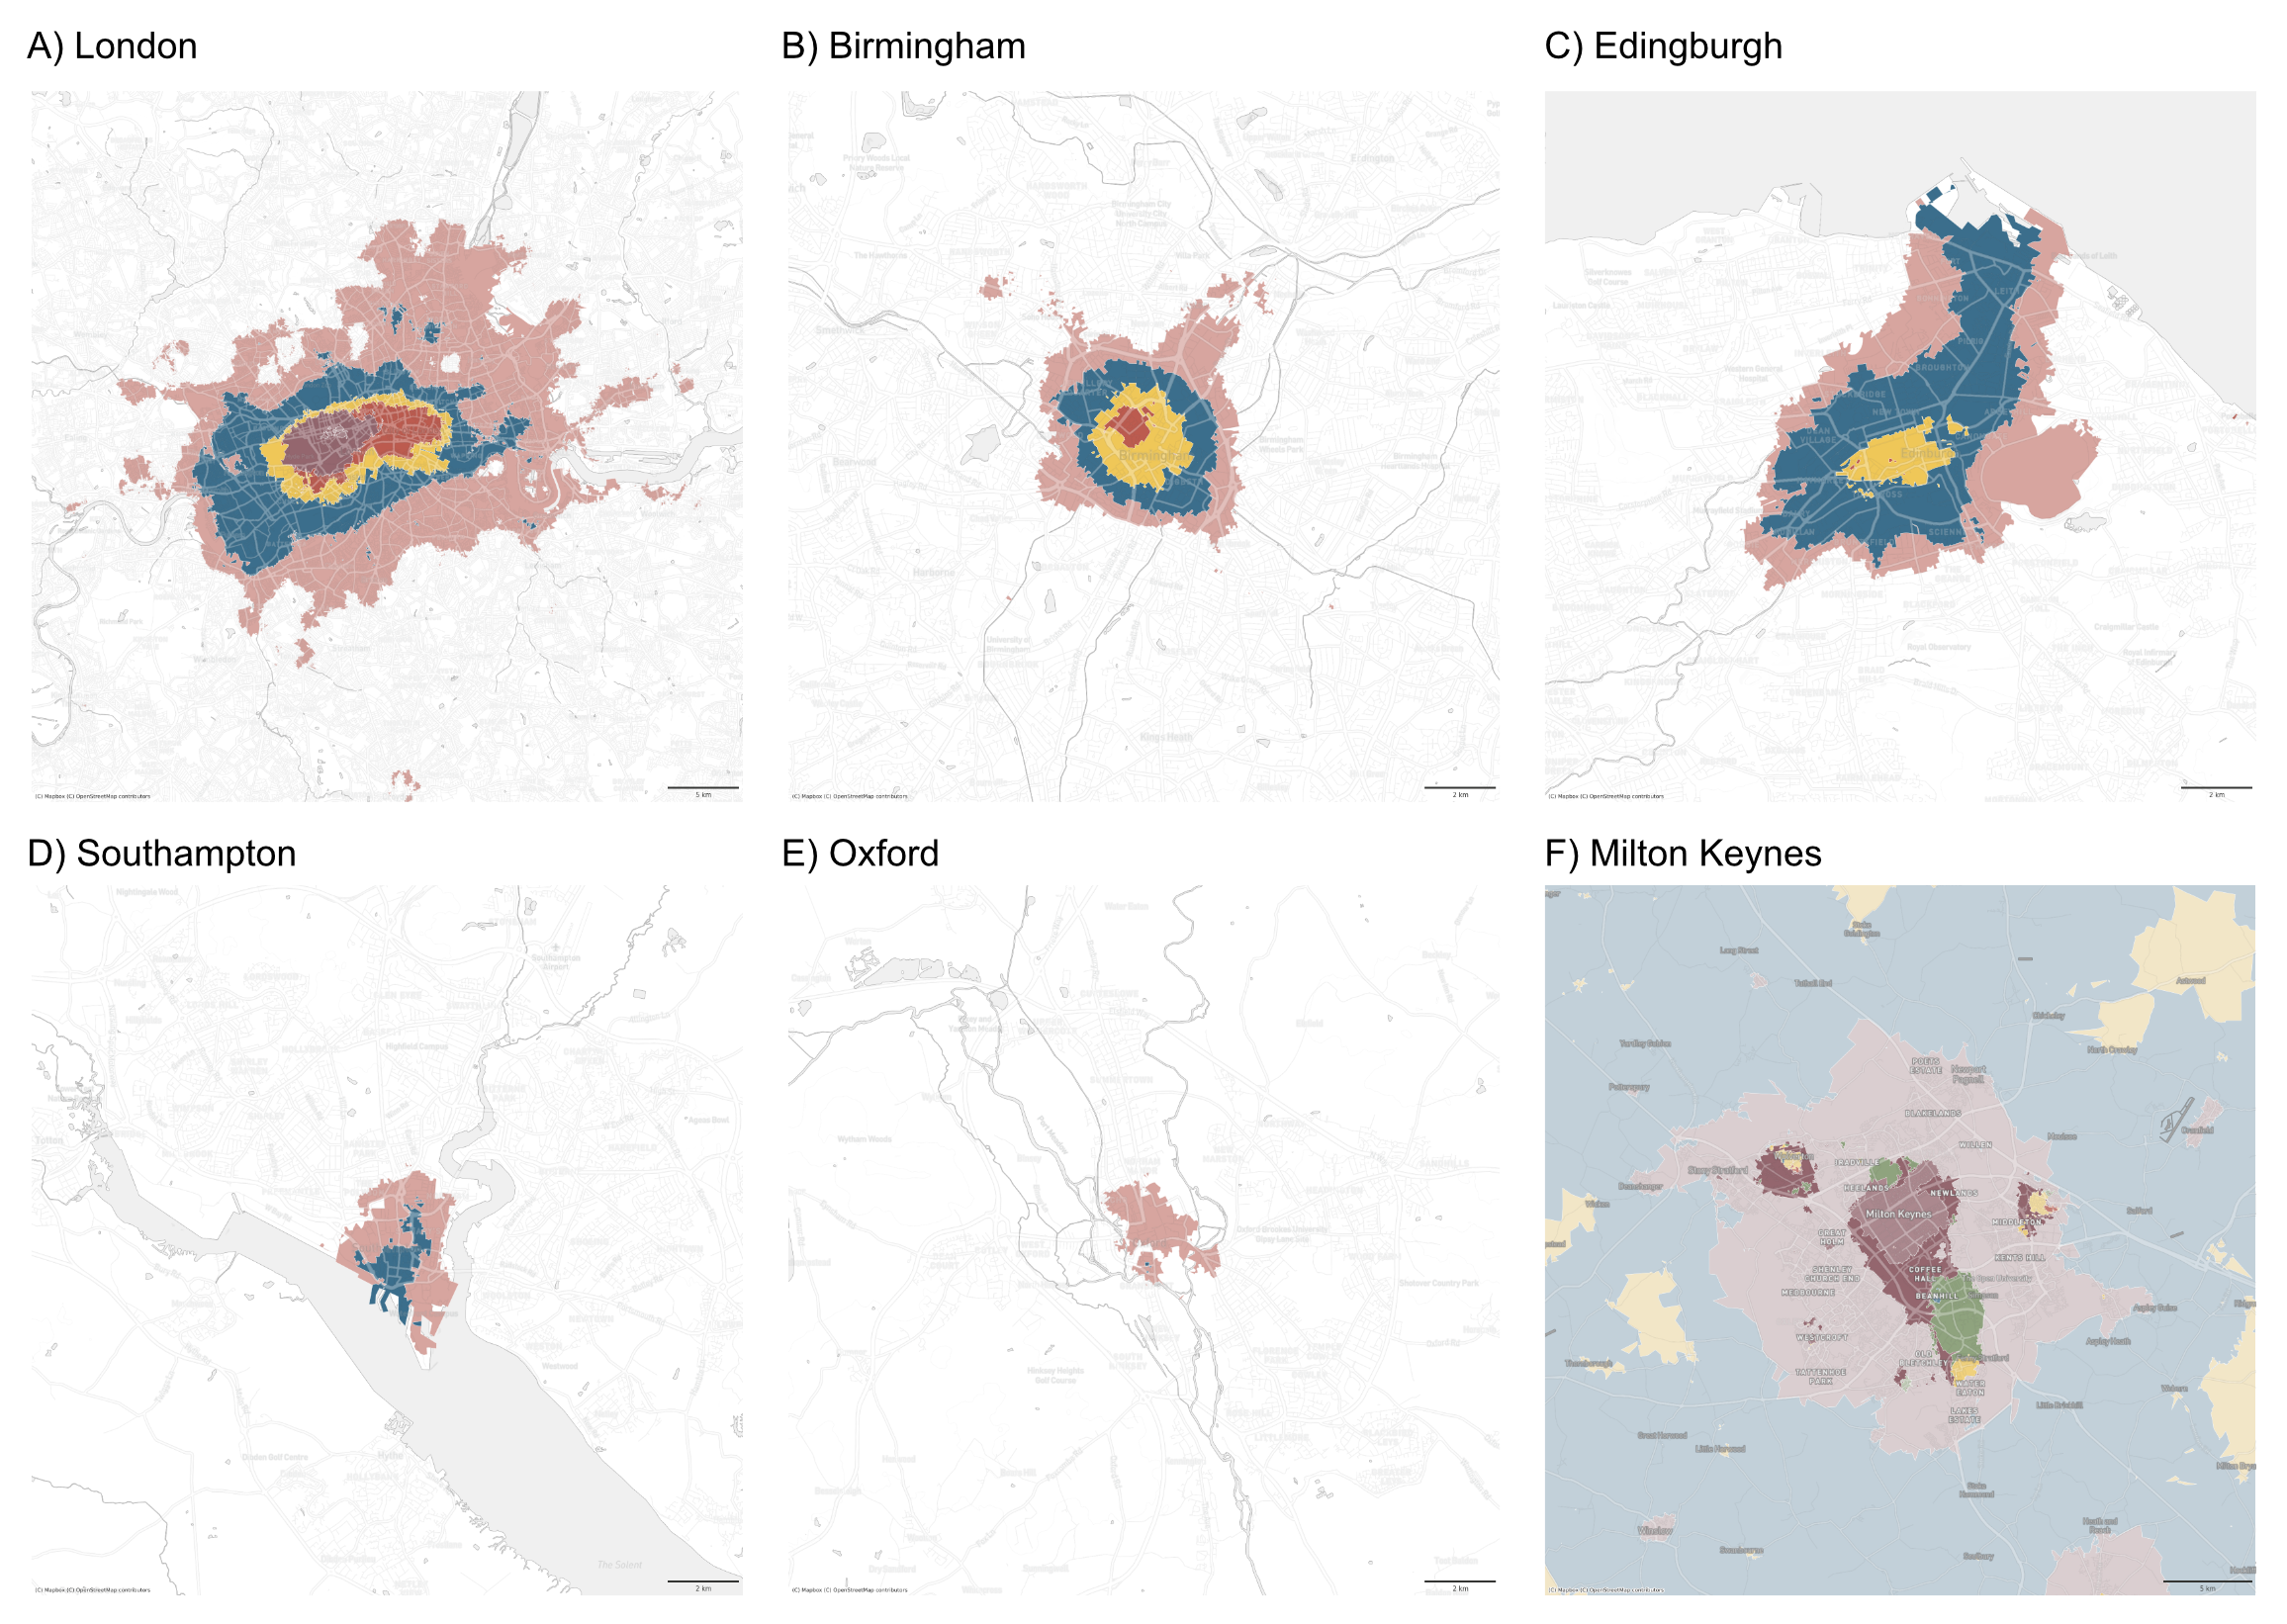
\includegraphics[width=0.75\linewidth, center]{fig/centres.png}
    \caption{Hierarchy of city centres from the most urban with all six morphosignature types
    belonging to city centres macro class in London (A), four types in Birmingham (B),
    three in Edinburgh (C), two in Southampton (D) and one in Oxford (E). Milton Keynes
    (F) does not have an area classified as morphological centre. Contains OS data © Crown copyright and database right 2021.}
    \label{fig:centres}
\end{figure}

% -- Milton Keynes does not have a morphological centre
Notable is the case of Milton Keynes, a new town built since 1960s on the green field
with a target population of 250 000 (currently at 230 000). Its development followed a
carefully designed masterplan, laying out the whole city. However, the resulting
structure is very different from any other city in the country as none of the morphosignatures
encoding urban centre is not present in Milton Keynes. We could say that it does not
have a morphologic centre, as illustrated on the Figure \ref{fig:centres}F.
